  %%%%%%%%%%%%%%%%%%%%%%%%%%%%%%%%%%%%%%%%%%%%%%%%%%%%%%%%%%%%%%%%%%%%%%
% LaTeX Example: Project Report

%%% Preamble
\documentclass[paper=a4, fontsize=11pt]{scrartcl}
\usepackage[T1]{fontenc}
\usepackage{fourier}
\usepackage{tabularx}
\usepackage[utf8]{inputenc}
\usepackage{hyperref}





\usepackage{listings}
\usepackage{color}

\definecolor{dkgreen}{rgb}{0,0.6,0}
\definecolor{gray}{rgb}{0.5,0.5,0.5}
\definecolor{mauve}{rgb}{0.58,0,0.82}
\lstset{frame=tb,
  language=[Visual]C++,
  aboveskip=3mm,
  belowskip=3mm,
  showstringspaces=false,
  columns=flexible,
  basicstyle={\small\ttfamily},
  numbers=none,
  numberstyle=\tiny\color{gray},
  keywordstyle=\color{blue},
  commentstyle=\color{dkgreen},
  stringstyle=\color{mauve},
  breaklines=true,
  breakatwhitespace=true,
  tabsize=3
}
\usepackage{graphicx}
\usepackage{caption}
\usepackage{subcaption}

\usepackage[english]{babel}															% English language/hyphenation
\usepackage[protrusion=true,expansion=true]{microtype}	
\usepackage{amsmath,amsfonts,amsthm} % Math packages

\usepackage{url}
%\usepackage[hang, small,labelfont=bf,up,textfont=it,up]{caption}


%%% Custom sectioning
\usepackage{sectsty}
\allsectionsfont{\normalfont\scshape}
\usepackage{float}
\usepackage{amsmath}
\usepackage{mathtools}



%%% Custom headers/footers (fancyhdr package)
\usepackage{fancyhdr}
\pagestyle{fancyplain}
\fancyhead{}											% No page header
\fancyfoot[L]{}											% Empty 
\fancyfoot[C]{}											% Empty
\fancyfoot[R]{\thepage}									% Pagenumbering
\renewcommand{\headrulewidth}{0pt}			% Remove header underlines
\renewcommand{\footrulewidth}{0pt}				% Remove footer underlines
\setlength{\headheight}{13.6pt}


%%% Equation and float numbering
\numberwithin{equation}{section}		% Equationnumbering: section.eq#
\numberwithin{figure}{section}			% Figurenumbering: section.fig#
\numberwithin{table}{section}				% Tablenumbering: section.tab#


%%% Maketitle metadata

\newcommand{\horrule}[1]{\rule{\linewidth}{#1}} 	% Horizontal rule

\title{
		%\vspace{-1in} 	
		\usefont{OT1}{bch}{b}{n}
		\normalfont \normalsize \textsc{} \\ [25pt]
		
\includegraphics[width=0.5\linewidth]{tri} \\
		%
\includegraphics[width=0.4\linewidth]{tru}		
		\horrule{0.5pt} \\[0.2cm]
		\huge M9 SiPM Spectrometer \\
		\horrule{2pt} \\[0.005cm]
}
\author{
		\normalfont 								\normalsize
        Jerin Roberts\\[-5pt]		\normalsize
        \today
}
\date{}




%%% Begin document
\begin{document}
\maketitle
\begin{center}
\begin{tabular}{l r}


Supervisor: & Dr. Syd Kreitzman  \\ % supervisor
Locations: & TRIUMF


\end{tabular}
\end{center}
\newpage
\tableofcontents
\listoffigures
\listoftables
\newpage
\lstset{language=[Visual]C++}

\section{Simulation}
\subsection{Introduction}
A large portion of work complete on this project involved simulating the effects of geometry and discrimination on timing. A multi-threaded simulation was written from scratch in c++, analyzed using ROOT and visualized using a simple openGL application. The simulation was designed to incorporate more geometrically complex scintillation pieces. This portion describes the simulations in detail for future modification ability. For the purpose of clarity each single SiPM device will be referred to as a "pixel" while each pixel on the device will be referred to as "micro-pixels" (Sensl convention). The simulation with installation instructions for linux machines is available on my github: \textit{https://github.com/j16out/scintS}

\subsection{Program Layout}
 The simulation is divided into three essential scripts. The Upper layer most commonly referred to as the 'macro level' uses a subset of functions found in the two lower levels. The layout of the simulation run is defined in the upper macro layer. Although the simulation consists of approximately 8000 lines of code, the user only deals with 20-30, depending on their needs. Below describes the list of functions one would call in a typical run for a macro.
\begin{lstlisting}
//-----------loading model-------------//
    load_geometry(scintsurf, "Project1");//geometry
    load_sensors(sensorsurf, "Project1");//sensors

//-----------Generating Scintillation-------------//

    scintillation = getscintpath(scintsurf, 5000, 1.0, 1.0, 2.0, points, "Project1");

//-----------Propagating/Detecting Photons-------------//

    getphoton(AFpath, pathtime, scintsurf, sensorsurf, scintillation, sensindex);	     	

//-----------OpenGl visualization---------//

	Tanimate(AFpath);//reorganize for fancy animation
	res = cadpath(AFpath);//generate file for opengl

//-----------ROOT analysis-----------// 

	TApplication theApp("App", &argc, argv);
	SignalTime(pathtime, sensindex);
	visroot(scintillation,sensorsurf,scintsurf,AFpath,pathtime);
	theApp.Run();

//-----------End Sim-----------//

\end{lstlisting} 
The files gPT and mROOT are the two lower level includes. gPT contains are relevent simulation and mathematical functions. The mROOT files contain all functions related to histogram and signal analysis via ROOT.

\subsection{Creating Geometry and Sensors}
The main feature of this simulation is its ability to quickly import new geometry and sensors via .ast (STL) generated cad files. The geometry is created using any capable modeler. For a open-source parametric modeler FreeCAD was used, available for all platforms. The simulation will use the imported geometry as the reflective layer to accurately propagate photons internally through the piece. When designing geometry there are some things to consider. Speed is a huge factor, although the sim is multi-threaded, its speed is determined by the size of the imported geometry. More vertices means longer sim times. So avoid filleting edges unless absolutely necessary.

\begin{figure}[h!]
\centering
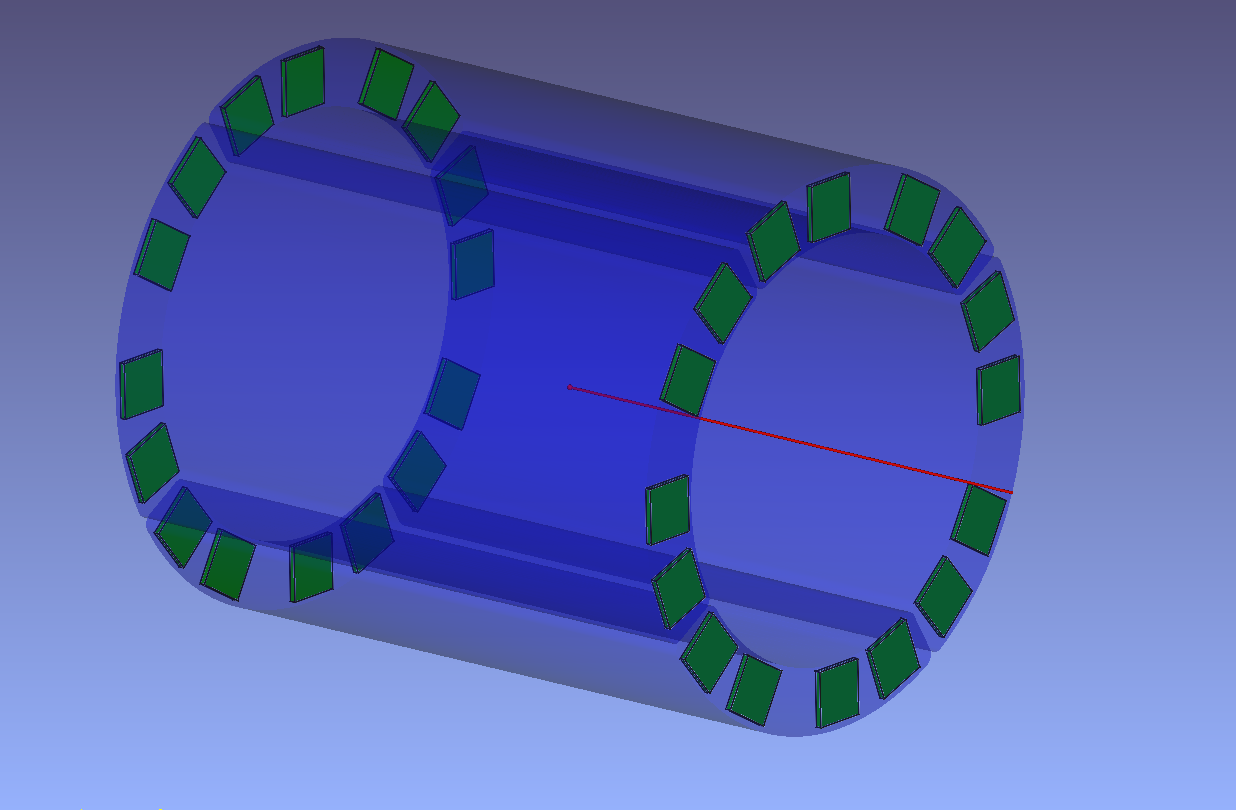
\includegraphics[width=0.70\linewidth]{fcad}
\caption{Displays an example of geometry (clear blue) and sensors (green) created using freecad.}
\label{geosens}
\end{figure}

 When generating mesh, be mindful of what density of vertices is required for your application. Obviously a higher density mesh will be more realistic and provide better accuracy as it more accurately represents a curved surface, however its at the expense of longer simulation times. The simulation requires two imports, one for geometry and the other for sensors. Sensors are imported the same way the geometry is using the
 \begin{verbatim}
  load_geometry("3D vector", "Project Directory")
  load_sensors(3D vector", "Project Directory") 
 \end{verbatim} 

 functions provided by gPT includes. The load functions require a 3D vector and the path of the project directory.The 3D vector will be filled with the vertice information from both the sensors and geometry. Figure \ref{geosens} displays an example of a geometry/sensor (G/S) set created using freeCAD. The simulation requires a ascii stereo-lithography file denoted '.ast' which contains all vertice and facet data. The simulation will use this data to build boundaries that will affect propagating photons.  The simulation requires a 'Project' folder which needs a specific layout. A directory for geometry and sensors are required. Geometry and Sensor .ast files are required to be labeled as g1 and s1 respectively. For designs requiring multiple G/S's models are to be named in succession and placed in the G/S directories. Ie A design with 4 sensors will require a sensor directory with 4 models labeled s1, s2, s3 and s4. When the simulation uploads the sensors an index will be generated keeping track of which detectors are stimulated. If one wishes to sum 4 sensors they should all be exported in the same .ast files ie only one sensor file (s1).
 

\subsection{Positron Generation}
Once geometry and sensors are imported into the simulation, the starting points of the photons need to be generated, ie positron generation. Start points are randomly produced along a trajectory set by the positron generator function. In addition random directions for photon propagation are also generated in this step. all are stored for later use in a 2D vector. For visualization the trajectory is used to manipulate a 'positron path' model used in the openGL visualization. The is all accomplished by retrieving the randomly generated data via the 
\begin{verbatim}
  getscintpath()
  getlaserpulse()
 \end{verbatim} 
functions, One for scintillation signal and laser signal respectively. When setting a positron or laser pulse trajectory its imperative to ensure it intercepts a scintillation piece. The path is able to intercept multiple pieces without any problem as displayed in figure \ref{multscint}, however its imperative the positron begin outside of the geometry, as it uses a primitive indexing system to know whens its inside or outside the scintillation piece ie its needs to intercept two surfaces to register a single scintillator piece. So if the positron begins inside the scintillator the simulator will only see it intercept one surface, and therefore will not register as a scintillating event and subsequently an error will occur. 

\begin{figure}[h!]
\centering
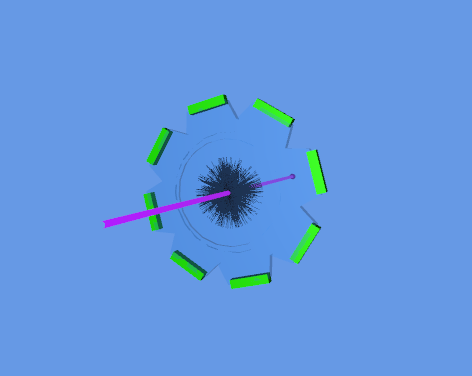
\includegraphics[width=0.70\linewidth]{posi2.png}
\caption{Displays simulated photon paths (black traces) originating from positron path (purple) and propagating to sensor (green).}
\label{simpic}
\end{figure}

\begin{figure}[h!]
\centering
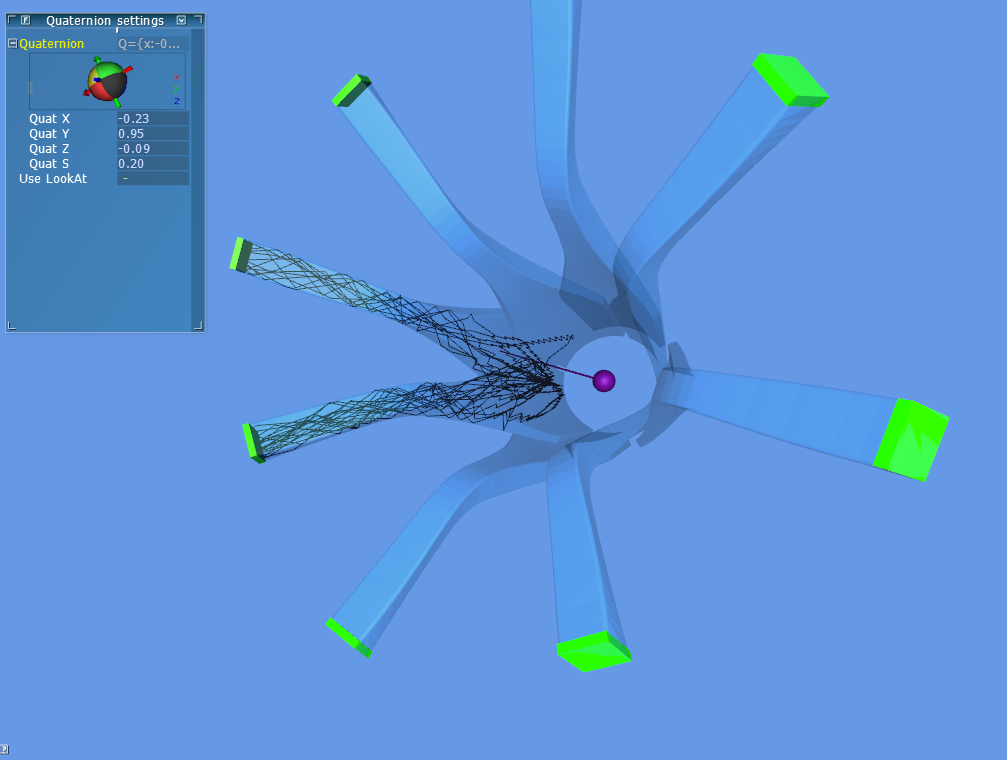
\includegraphics[width=0.70\linewidth]{posi3.png}
\caption{Displays the programs ability to simulate complex scintillation structures.}
\label{simpic}
\end{figure}

\begin{figure}[h!]
\centering
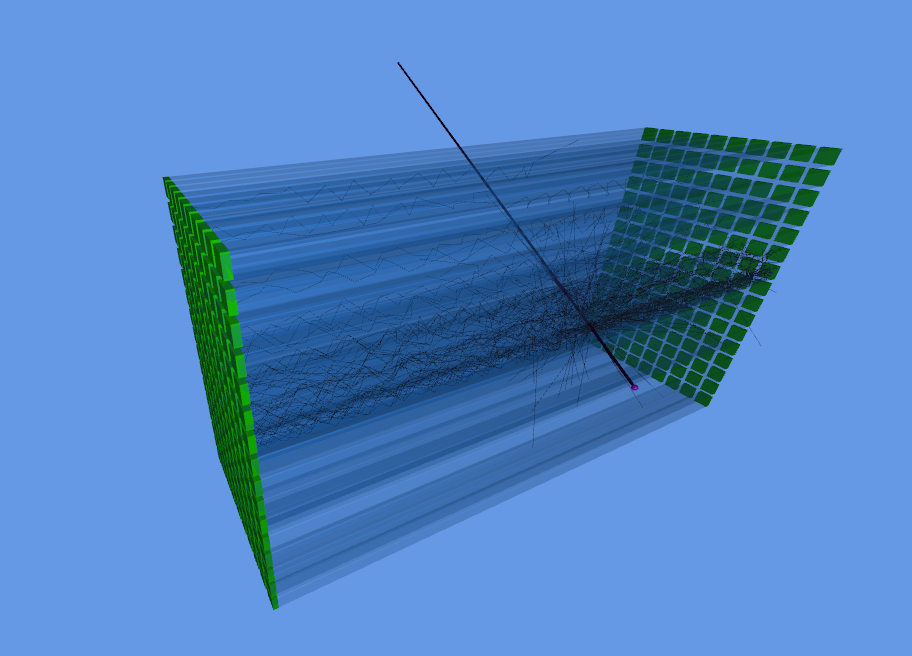
\includegraphics[width=0.70\linewidth]{multscint.png}
\caption{Displays the multiple intercept capabilities of the simulator. Positron intercepts multiple pieces producing scintillating photons in each.}
\label{multscint}
\end{figure}

\subsection{Photon Propagation}
Photons are permitted to propagate from the point of origin until a boundary is reached. The scintillator boundary is defined by cluster of interlocking triangles, ie a mesh. If the photon intersects the boundary then it must intercept one of these triangles that make up the surface. The simulator imports the .ast mesh file and builds a vector of triangles which makes up the surface. Once a photons random direction is selected, an algorithm is used to check to see if it intercepts any of the triangles along its path of flight. If an intersection is detected, a intercept point, and reflected vector are calculated and the simulation begins rechecking for triangle intercepts using the new reflected direction. This process yields the path of the photon and subsequently the time of flight as it propagates through the scintillation piece. 

The Algorithm employed is nearly identical to the Ray and triangle intersection computation that is used in computer graphics rendering programs. Assume we have a ray $R$ going from points $P_0$ to $P_1$, and a plane P through $V_0$ with normal $n$. The parametric line $L$ denoted as $P(r)=P_0+r(P_1-P_0)$ and intersects the plane $P$ at the point $P(r_I)$ with parameter value:


\begin{equation}
\label{rI}
r_I=\frac{n\cdot(V_0-P_0)}{n\cdot(P_1-P_0)}
\end{equation}

When the denominator $n\cdot(P1-P0)=0$, the line $L$ is parallel to the plane $P$ , and thus either does not intersect it or else lies completely in the plane (whenever either P0 or P1 is in P ). Otherwise, when the denominator is nonzero and $r_I$ is a real number, then the ray $R$ intersects the plane P only when $r_I\geq0$. A segment S intersects P only if $r_I\geq0\leq1$. In all algorithms, the additional test $r_I\leq1$ is the only difference for a segment instead of a ray.
Intersection of a Ray/Segment with a Triangle

Consider a ray R from $P_0$ to $P_1$, and a triangle T with vertices $V_0$, $V_1$ and $V_2$. The triangle $T$ lies in the plane $P$  through $V_0$ with normal vector $n=(V_1-V_0)\times(V_2-V_0)$. To get the intersection of R with T, one first determines the intersection of R and P . If it does not intersect, then it also does not intersect T and we are done. However, if they intersect in the point $PI = P(rI)$, we need to determine if this point is inside the triangle T for there to be a valid intersection.

 The parametric plane equation is given by:
 
 \begin{equation}
\label{vsl}
V(s,t) = V_0+s(V_1-V_0)+t(V_2-V_0) = V_0+su+tv
\end{equation}

where $u=V_1-V_0$ and $v=V_2-V_0$ are edge vectors of T. Then, $P=V(s,t)$ is in the triangle T when $s\geq0$, $t\geq0$, and $s+t\leq1$. So, given $P_I$, one just has to find the $(s_I, t_I)$ coordinate for it, and then check these inequalities to verify inclusion in T. Further, $P=V(s,t)$ is on an edge of T if one of the conditions $s = 0$, $t = 0$, or $s + t = 1$ is true (each condition corresponds to one edge). And, the three vertices are given by: $V_0=V(0,0)$, $V_1=V(1,0)$, and $V_2=V(0,1)$.

\begin{figure}[h!]
\centering
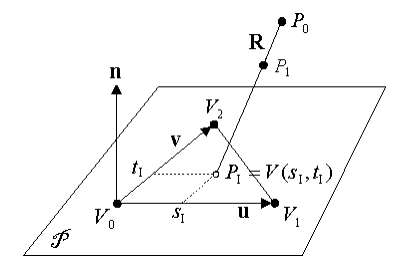
\includegraphics[width=0.5 
\linewidth]{alg.png}
\label{alg}
\end{figure}

There all that is left is to find $s_I$ and $t_I$.  With $w=P_I-V_0$, which is a vector in P  (that is, $n\cdot(w)=0$), we solve the equation: $w=s_u+t_v$ for s and t. The final result is:

 \begin{equation}
\label{fs}
s_I= \frac{(u\cdot v)(w\cdot v)-(v\cdot v)(w\cdot u) }{(u\cdot v)^2-(u\cdot u)(v\cdot v)}
\end{equation}

 \begin{equation}
\label{ft}
t_I= \frac{(u\cdot v)(w\cdot u)-(u\cdot u)(w\cdot v) }{(u\cdot v)^2-(u\cdot u)(v\cdot v)}
\end{equation}

which has only 5 distinct dot products. It has been arranged in terms so that the two denominators are the same and only need to be calculated once.

When the geometry and Sensors are loaded and a positron path has been defined photon propagation can be iterated. Using the algorithm described above photon travel times are calculated from start until its reaches a sensor. Photons that encounter boundaries at angle below the critical angle (relative to normal) will transmit out of the scintillator, these photons are stopped and times are discarded. If the 'RT' code is used a transmitted path will be loaded into the openGL visualizer (default). Reverting to 'R' code will only display internally reflected photons. Photons that arrive at the sensor surface at angle greater than critical angle (relative to normal) are also discarded as the photon would not transmit into the detector. The critical angle can be adjusted inside the gen() function called by the multi-threading method getphoton().



\subsection{Final Signal}
In addition to providing the distribution of arrival times the final signal from each sensor is calculated. This is done by summing all the individual micro-pixel signals with the timing adjustment, which is denoted as $t_o$ in equation \ref{risefall}.



\begin{equation}
\label{risefall}
V(t) = V_{max} (exp(\frac{-(t-t_{o})}{\tau_{Rise}})-exp(\frac{-(t-t_{o})}{\tau_{Fall}}))
\end{equation}

The program applies each timing adjustment before summing all the signals. The signals are summed and stored in a vector. The size of the vector denotes the resolution of the signal, ie each component of the vector represents a point in the final function. Initially the entire vector is set to zero. Then the timing adjustment is imputed into a function which is then evaluated for each component in the vector. The process continues for each timing adjustment as shown below.

\begin{lstlisting}
for(int n = 0; n < ftime.size(); ++n)
	{
	for(int i = 0; i < graphs1A.size(); ++i)
		{
			tomp = -(11.94)*(exp(-((i*.001)-ftime.at(n))/2.341)-exp(-((i*.001)-ftime.at(n))/9.526));
			if (tomp > 0)
			{
				if(Sfinpos1.at(n) == 1)
				graphs1A.at(i) = tomp + graphs1A.at(i);
				if(Sfinpos1.at(n) == 2)
				graphs1B.at(i) = tomp + graphs1B.at(i);
				if(Sfinpos1.at(n) == 3)
				graphs1C.at(i) = tomp + graphs1C.at(i);
				if(Sfinpos1.at(n) == 4)
				graphs1D.at(i) = tomp + graphs1D.at(i);
			}
			else
			{
				if(Sfinpos1.at(n) == 1)
				graphs1A.at(i) = 0 + graphs1A.at(i);
				if(Sfinpos1.at(n) == 2)
				graphs1B.at(i) = 0 + graphs1B.at(i);
				if(Sfinpos1.at(n) == 3)
				graphs1C.at(i) = 0 + graphs1C.at(i);
				if(Sfinpos1.at(n) == 4)
				graphs1D.at(i) = 0 + graphs1D.at(i);
			
			}
		}
}
\end{lstlisting}

 This makes for an efficient and memory saving method for calculating the final function. There are a couple of lines which organize all timings into specific groups corresponding to different pixels. These final signals are then shifted based on a threshold, then the intercept is calculated. This gives the timing of the applied threshold. These are saved from each signal then checked for coincidence. If all signals from each pixel are above threshold, then the earliest time is stored. If one signal is not above threshold the entire run is discarded. The earliest signal from each end of the scintillator is then saved and used for statistics. The simulation will then reset for another event. The results of all the events are tallied and used to determine the timing resolution of the experiment. figure \ref{simd1}  is an example of the final output for the simulation. In addition to the final data being saved in '.root' files, a log of the simulation is stored in '.txt' for future analysis or debugging.

 
 \begin{figure}[H]
\centering
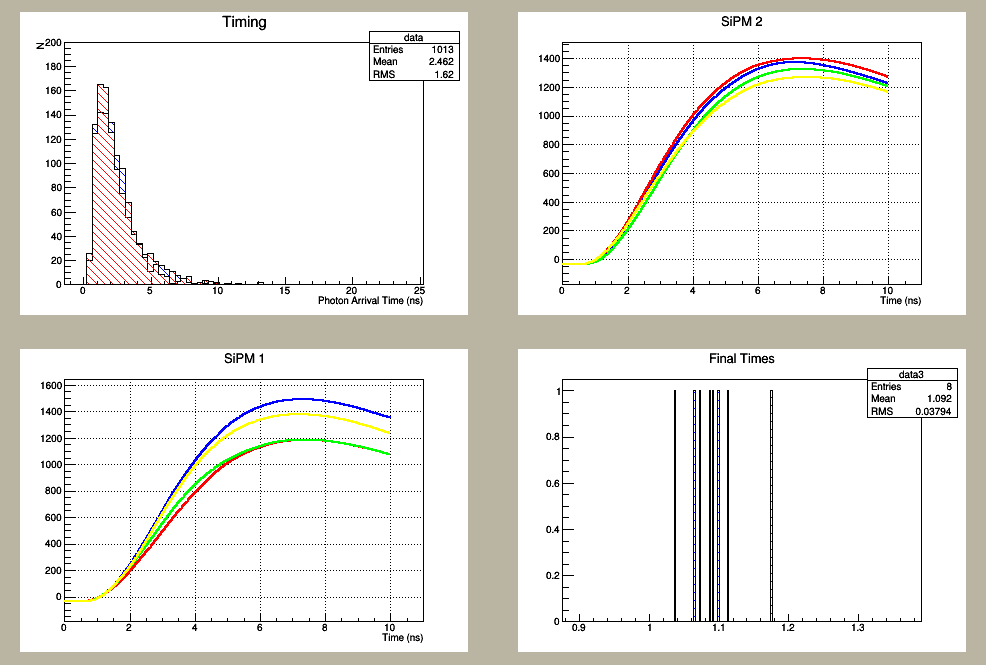
\includegraphics[width=0.80\linewidth]{simd1}
\caption{Displays a sample output of the simulator. The first graph shows all timings, the 2nd and 3rd show the final signals from each array, while the last shows the results of threshold timing.}
\label{simd1}
\end{figure} 
\newpage
\newpage
\newpage





%%% End document
\end{document}